%%MaD.tex - Notes taken for Materials and Devices Lecture
%%Author: Andy Goetz
%%Date Modified: 10-7-09
%%License: Ask me before reproducing/modifying, etc.


\documentclass{article}

%Make sure you have the file ShumanNote.scy in the same directory as
%this one. It has contains the style sheet for ECE111, and is needed
%to standardize the layout of LateX documents created for the class.
\usepackage{ShumanNotes} 
\usepackage{tikz}
\usepackage{program}
\usepackage{listings}
\pdfpagewidth 8.5in 
\pdfpageheight 11in

%This package is used to line up pictures 
\usepackage{graphicx}
\usepackage{fancyvrb}
\usepackage{listings}
%allows cursive font
%\usepackage{amsmath}

%allows hyperlinks 
%\usepackage{hyperref}

\newcommand{\HRule}{\rule{\linewidth}{0.5mm}} 

\lhead{Homework 5}

\begin{document}

%% These commands allow me to use cursive letter for things such as
%% length.  Note that on ubuntu linux, this required installation of
%% the package 'texlive-fonts-extra'. 
%% Taken from
%% http://www.latex-community.org/forum/viewtopic.php?f=5&t=1404&start=0
\newenvironment{frcseries}{\fontfamily{frc}\selectfont}{}
\newcommand{\textfrc}[1]{{\frcseries#1}}
\newcommand{\mathfrc}[1]{\text{\textfrc{#1}}}

\section{Overview}
The T-16 Audio Synthesizer is designed to generate an audio output based on multiple channel inputs, as well as tuneable parameters that are controllable from the user interface.  The functionality can be broken down into several independent sub-modules.  These include a microcontroller to synthesize the audio signal, as well as act as a central communications hub for the other sub-modules, a regulated power supply, an EEPROM memory to dynamically store and load pre-defined user settings and miscellaneous data, an LCD to present the user interface, a DAC to convert the synthesizer's digital audio samples into an analog audio output, and an audio amplifier to provide more output power to an internal speaker and offer a master volume control.

\section{T-16 Audio Synthesizer Level 0 Diagram}
\centerimage{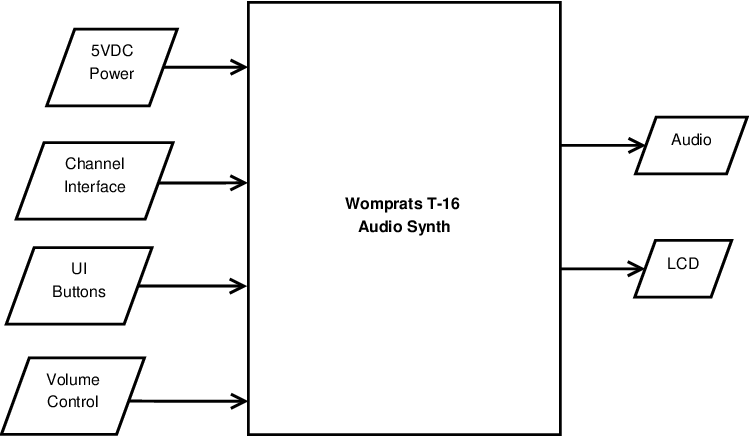
\includegraphics[width=5in]{synth0.png}}{Level 0 Diagram}{fullzero}

\begin{tabular}{|p{1in}|p{5in}|}
\hline
\emph{Module} & T-16 Audio Synthesizer \\
\hline
\emph{Inputs}& 5VDC Power: Unregulated 5 VDC power from a wall-wart power supply.\\
	     & Channel Interface: Six analog/digital paired signals that modify parameters that control the synthesizer software. \\
      	     & UI Buttons: Up/Down/Left/Right/Ok/Aux buttons that allow you to navigate the Menu UI on the LCD and modify tunable parameters in the synthesizer software.\\
	     & Volume Control: Master output volume control of the internal speaker.\\
\hline
\emph{Outputs}& Audio: Audio output generated by the audio synthesis software in the microcontroller.\\ 
	      & LCD: Shows the Menu user interface which presents the user with controllable parameters that affect the sound synthesis. It also presents the logo on startup. \\
\hline
\emph{Functionality}& Takes input from the channel interface as well as parameters set in the user interface, and synthesizes an audio waveform based on these inputs. This audio waveform is either output to an amplified internal speaker or an external line-out.\\
\hline
\end{tabular}

\section{T-16 Audio Synthesizer Level 1 Diagram}
\centerimage{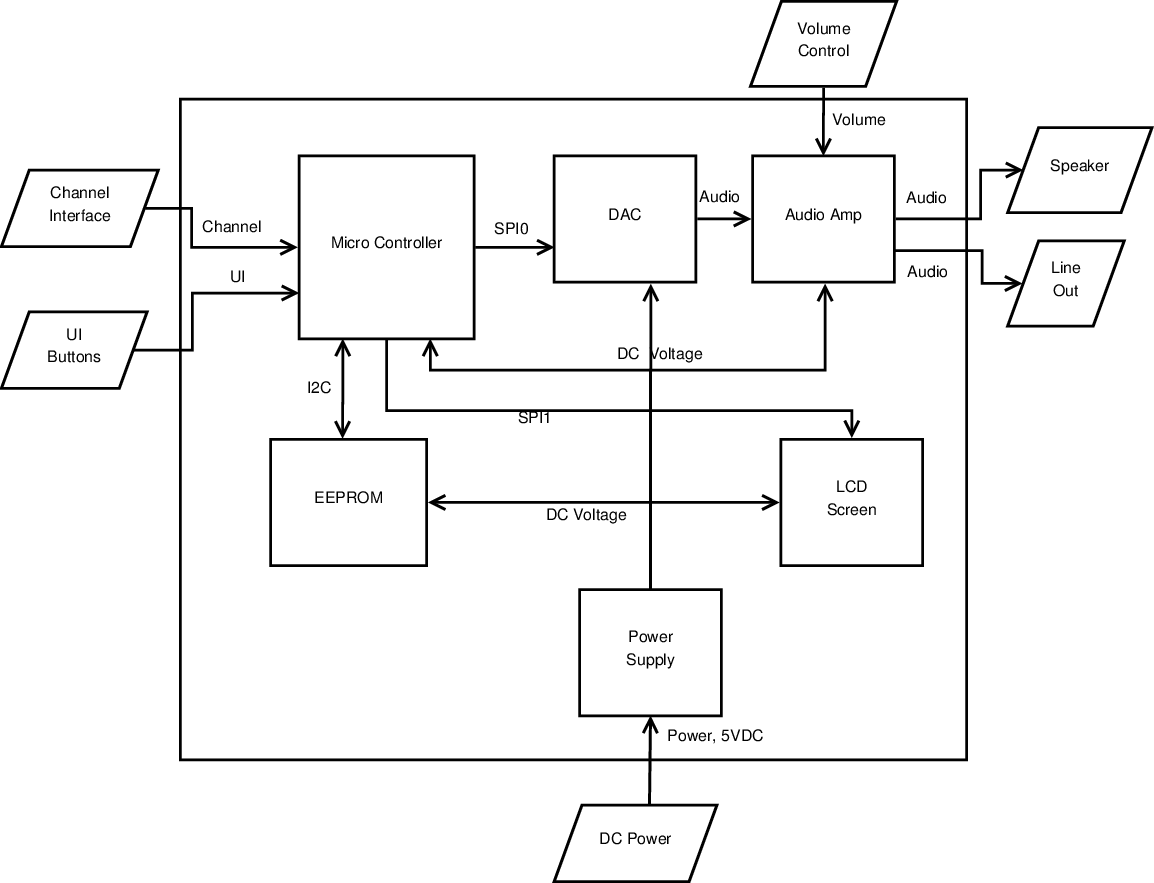
\includegraphics[width=5in]{synth1.png}}{Level 1 Diagram}{fullone}

\newpage

\section{LCD Level 0 Diagram}
\centerimage{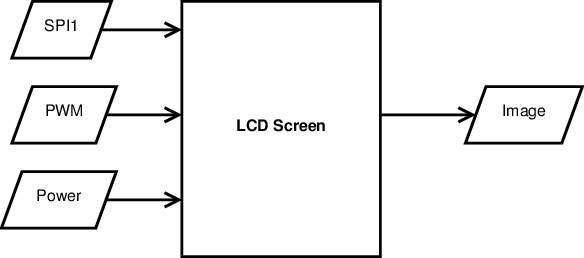
\includegraphics[width=5in]{lcd.png}}{Level 0 Diagram}{LCD}

\begin{tabular}{|p{1in}|p{5in}|}
\hline
\emph{Module} & LCD \\
\hline
\emph{Inputs}& SPI: Receives image data from microcontroller.\\
	     & PWM: Backlight brightness control 0-100\% duty cycle.\\
	     & Power: 3.3 VDC Power.\\
\hline
\emph{Outputs}& Image: Black and white image on 102x64 raster LCD.\\
	      & Backlight: LED light to illuminate the LCD.\\ 
\hline
\emph{Functionality}& Display the user interface and state of the synthesizer.\\
\hline
\end{tabular}

\section{Power Supply Level 0 Diagram}
\centerimage{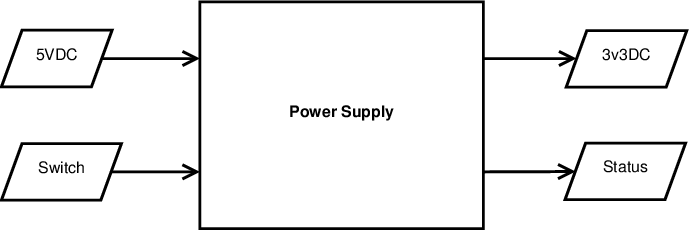
\includegraphics[width=5in]{pwrsply.png}}{Level 0 Diagram}{PSU}

\begin{tabular}{|p{1in}|p{5in}|}
\hline
\emph{Module} & Power Supply \\
\hline
\emph{Inputs}& 5VDC: Unregulated power from 5 VDC wall-wart power supply.\\
	     & Switch: On/Off Power Switch.\\
\hline
\emph{Outputs}& 3v3DC: Regulated 3.3 VDC Power.\\
	      & Status: LED to display if the input power is available.\\ 
\hline
\emph{Functionality}& The power supply provides regulated 3.3 VDC power to all the subsystems of the audio synthesizer.\\
\hline
\end{tabular}

\section{EEPROM Level 0 Diagram}
\centerimage{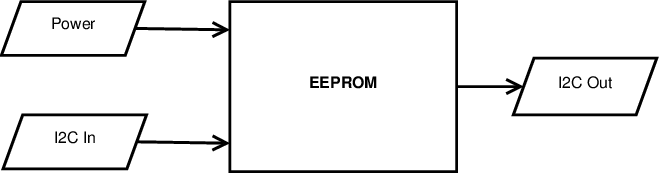
\includegraphics[width=5in]{eeprom.png}}{Level 0 Diagram}{eeprom}

\begin{tabular}{|p{1in}|p{5in}|}
\hline
\emph{Module} & EEPROM \\
\hline
\emph{Inputs}& Power: 3.3 VDC Power\\
	     & I2C In: Read data from microcontroller \\
\hline
\emph{Outputs}& I2C Out: Write data to microcontroller \\ 
\hline
\emph{Functionality}& Holds user settings for the synthesizer state, as well as the Womprats logo for startup\\
\hline
\end{tabular}

\section{Microcontroller Level 0 Diagram}
\centerimage{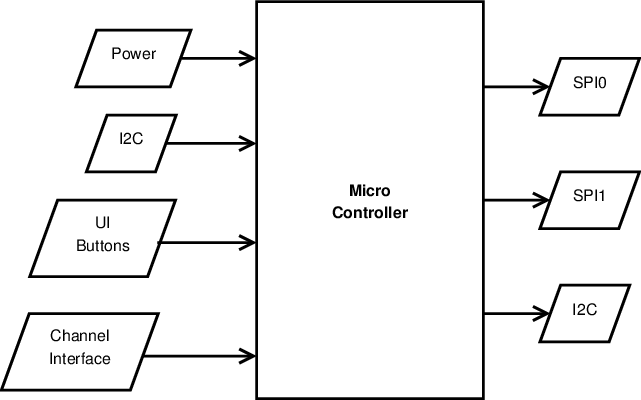
\includegraphics[width=5in]{microcont.png}}{Level 0 Diagram}{micro}

\begin{tabular}{|p{1in}|p{5in}|}
\hline
\emph{Module} & Microcontroller \\
\hline
\emph{Inputs}& Power: 3.3 VDC Power\\
	     & I2C: Retrieve data stored in EEPROM\\
	     & UI Buttons: Up/Down/Left/Right/OK/Aux button controls for UI menu interface and entering audio synthesizer settings.\\
	     & Channel Interface: Six analog and digital signal lines that supply parameter control to the audio synthesizer.\\
\hline
\emph{Outputs}& SPI$_0$: Send digital audio samples to DAC.\\
	      & SPI$_1$: Send image data to LCD.\\
	      & I2C: Store data in EEPROM.\\ 
\hline
\emph{Functionality}& Implements a software synthesizer that generates an audio signal, shows it's current settings via an LCD screen, is controllable through tunable parameters in the UI and from analog/digital signals on its channel inputs. The tunable parameters are stored in an EEPROM memory that is recalled on startup.\\
\hline
\end{tabular}

\section{DAC Level 0 Diagram}
\centerimage{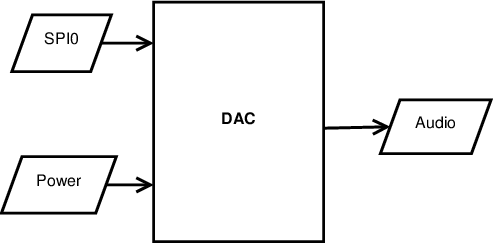
\includegraphics[width=5in]{dac.png}}{Level 0 Diagram}{dac}

\begin{tabular}{|p{1in}|p{5in}|}
\hline
\emph{Module} & DAC \\
\hline
\emph{Inputs}& SPI$_0$: Audio samples received from the microcontroller\\
	     & Power: 3.3 VDC power\\
\hline
\emph{Outputs}& Audio: 0-3.3V audio signal \\ 
\hline
\emph{Functionality}& The DAC takes the digital audio sample from the microcontroller and converts an analog 0-3.3V audio signal.\\
\hline
\end{tabular}

\section{Audio Amplifier Level 0 Diagram}
\centerimage{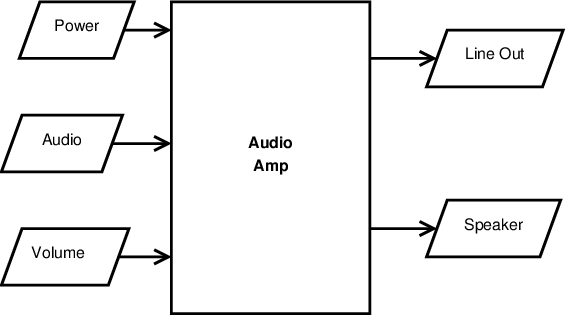
\includegraphics[width=5in]{audioamp.png}}{Level 0 Diagram}{audio}

\begin{tabular}{|p{1in}|p{5in}|}
\hline
\emph{Module} & Audio Amplifier \\
\hline
\emph{Inputs} & Power: 3.3 VDC Power\\
	      & Audio: 0-3.3V audio signal from DAC\\
	      & Volume: Controls the audio output volume. Logarithmic control.\\
\hline
\emph{Outputs}& Line out: Unamplified audio output to external line-out.\\ 
	      & Speaker: Amplified audio output to internal speaker.\\
\hline
\emph{Functionality}& Provide an amplified audio out that can be heard over the internal speaker or line-out to an external audio device.\\
\hline
\end{tabular}

\newpage

\section{EEPROM UML Use Cases}
\subsection{Introduction}


\subsection{Save Synth State}
\begin{tabular}{|p{1in}|p{5in}|}
\hline
\textbf{Use Case} & Save\\
\hline
\textbf{Description} & Saves the current synthesizer state into the synthesizer core memory.\\
\hline
\textbf{Actors} & I$^2$C, EEPROM, synthesizer core\\
\hline
\textbf{Assumptions} & There will be the correct amount of power supplied to the EEPROM and microcontroller.  In addition, there must be usable storage space to save in EEPROM.\\
\hline
\textbf{Steps} & \begin{enumerate}
\item Receive synth state data pointer from synth core.
\item Iterate over every byte of state data and send to the EEPROM via I$^2$C.
\end{enumerate}\\
\hline
\textbf{Issues} & Synth state has yet to be defined.\\
& Functionality has yet to be implemented.\\
& EEPROM memory map has yet to be defined.\\
\hline
\end{tabular}

\subsection{Load Synth State}
\begin{tabular}{|p{1in}|p{5in}|}
\hline
\textbf{Use Case} & Load\\
\hline
\textbf{Description} & Loads pre-saved synthesizer state into synthesizer core memory.\\
\hline
\textbf{Actors} & I$^{2}$C, EEPROM, synthesizer core\\
\hline
\textbf{Assumptions} & There will be the correct amount of power supplied to the EEPROM and microcontroller.  In addition, there will be a valid state to load.\\
\hline
\textbf{Steps} & \begin{enumerate}
\item Read synth state data from I$^2$C EEPROM.
\item Pass synth state data pointer to synth core.
\end{enumerate}\\
\hline
\textbf{Issues} & Synth state has yet to be defined.\\
& Functionality has yet to be implemented.\\
& EEPROM memory map has yet to be defined.\\
\hline
\end{tabular}

\subsection{Load Splash Screen Image}
\begin{tabular}{|p{1in}|p{5in}|}
\hline
\textbf{Use Case} & Splash Screen Image\\
\hline
\textbf{Description} & Loads the Womprats Logo splash screen into memory.\\
\hline
\textbf{Actors} & LCD driver, EEPROM, I$^2$C\\
\hline
\textbf{Assumptions} & There will be the correct amount of power supplied to the EEPROM and microcontroller.  In addition, the image bits to be loaded will always remain intact.\\
\hline
\textbf{Steps} & \begin{enumerate}
\item Read logo data from I$^2$C EEPROM.
\item Pass logo data to LCD driver
\end{enumerate}\\
\hline
\textbf{Issues} & How the logo data is loaded into EEPROM has yet to be determined.\\
& Functionality has yet to be implemented.\\
& EEPROM memory map has yet to be defined.\\
\hline
\end{tabular}

\section{EEPROM UML Interaction View}
\subsection{Save Synth State}
\centerimage{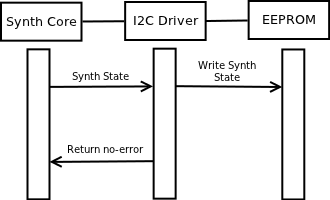
\includegraphics[width=5in]{SaveUML.png}}{Save Synth State}{}
\subsection{Load Synth State}
\centerimage{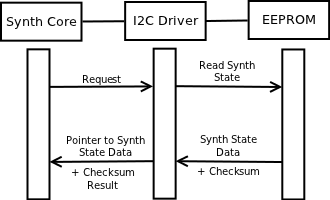
\includegraphics[width=5in]{LoadUML.png}}{Load Synth State}{}
\subsection{Load Splash Screen Image}
\centerimage{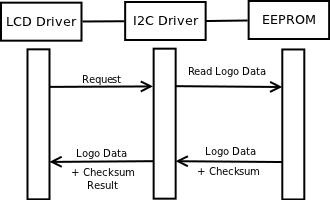
\includegraphics[width=5in]{logoLoadUML.png}}{Load Splash Screen}{}

\end{document}
